\documentclass[border=3pt,tikz]{standalone}
\usepackage{amsmath}
\usetikzlibrary{calc}
\usetikzlibrary{arrows.meta} % for arrow size
\begin{document}
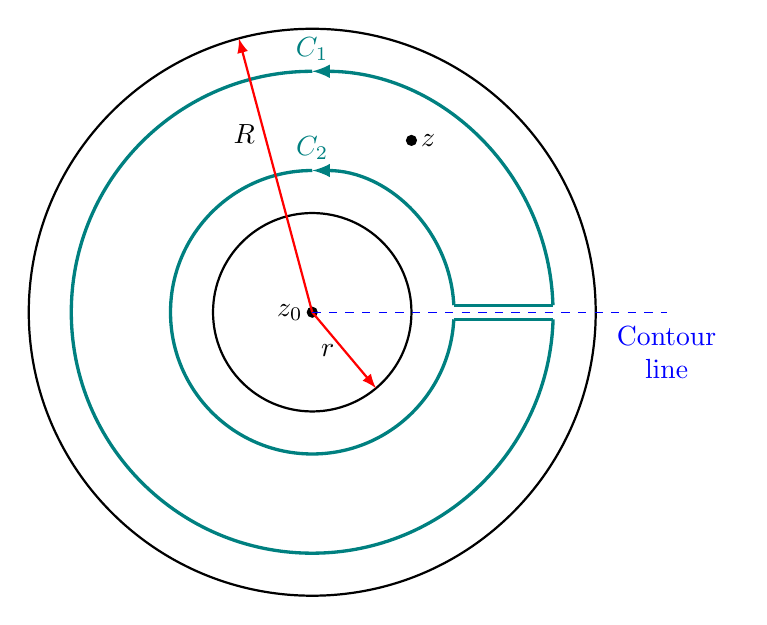
\begin{tikzpicture}[scale=1.8]
    \usetikzlibrary {arrows.meta}
    \usetikzlibrary {calc}
    
    \coordinate (p1) at (0.9987502603949663, 0.04997916927067833);
    \coordinate (p2) at (1.6978754426714426, 0.04997916927067833);
    \coordinate (q1) at (0.9987502603949663, -0.04997916927067833);
    \coordinate (q2) at (1.6978754426714426, -0.04997916927067833);
    
    
    
    \draw [thick] (0, 0) circle (0.7) ;
    \draw [thick] (0, 0) circle (2.0);
    \filldraw [] (0,0) circle (1pt) node [left] {$z_0$} ;
    \draw[teal, very thick] (p1) -- (p2);
    \draw[teal, very thick] (q1) -- (q2);
    \draw[teal, very thick, -latex] (p1) arc (2.865:90:1) node [above] {$C_2$};
    \draw[teal, very thick] (0, 1.0) arc (90:357.135:1);
    \draw[teal, very thick, -latex] (p2) arc (1.686:90:1.7) node[above] {$C_1$};
    \draw[teal, very thick] (0, 1.7) arc (90:358.314:1.7);
    
    \draw[red, thick, -latex] (0, 0) -- ({0.7*cos(310)}, {0.7*sin(310)});
    \node[left] at ({0.35*cos(310)}, {0.35*sin(310)}) {$r$};
    
    \draw[red, thick, -latex] (0, 0) -- ({2*cos(105)}, {2*sin(105)});
    \node[left] at ({1.3*cos(105)}, {1.3*sin(105)}) {$R$};
    
    \draw[dashed, blue] (0, 0) -- (2.5, 0) node[below] {$\begin{array}{cc}\text{Contour}\\ \text{line} \end{array}$};
    \filldraw[] ({1.4*cos(60)}, {1.4*sin(60)}) circle(1pt) node[right] {$z$};
    
    
    \end{tikzpicture}  
\end{document}